\documentclass[border=2pt]{standalone}
\usepackage{tikz}
\usetikzlibrary{arrows.meta, positioning, calc}
\usepackage{amsmath}

\begin{document}
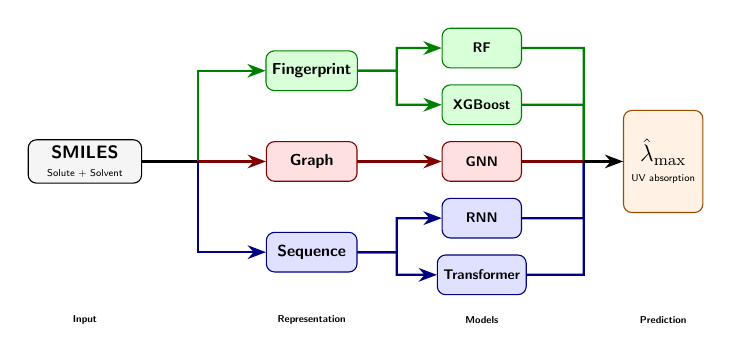
\begin{tikzpicture}[
    >=Stealth,
    scale=0.72, every node/.style={scale=0.72},
    box/.style={draw, rounded corners=3pt, align=center, font=\sffamily\small,
                inner sep=3pt, minimum height=0.7cm},
    arr/.style={->, thick},
]

% ---- Input ----
\node[box, fill=gray!8, draw=black, minimum width=2.0cm] (input) at (0, 0)
    {\textbf{SMILES}\\[-2pt]{\tiny Solute + Solvent}};

% ---- Three representation paths ----
\coordinate (fork) at (2.0, 0);
\draw[thick, draw=black] (input.east) -- (fork);

% Fingerprint path
\node[box, fill=green!15, draw=green!50!black, minimum width=1.6cm] (fp) at (4.0, 1.6)
    {\textbf{\footnotesize Fingerprint}};

% Graph path
\node[box, fill=red!12, draw=red!50!black, minimum width=1.6cm] (graph) at (4.0, 0)
    {\textbf{\footnotesize Graph}};

% Sequence path
\node[box, fill=blue!12, draw=blue!50!black, minimum width=1.6cm] (seq) at (4.0, -1.6)
    {\textbf{\footnotesize Sequence}};

\draw[arr, draw=green!50!black] (fork) |- (fp.west);
\draw[arr, draw=red!50!black] (fork) -- (graph.west);
\draw[arr, draw=blue!50!black] (fork) |- (seq.west);

% ---- Models (more vertical spacing) ----
\node[box, fill=green!15, draw=green!50!black, font=\sffamily\scriptsize, minimum width=1.4cm] (rf) at (7.0, 2.0) {\textbf{RF}};
\node[box, fill=green!15, draw=green!50!black, font=\sffamily\scriptsize, minimum width=1.4cm] (xgb) at (7.0, 1.0) {\textbf{XGBoost}};
\node[box, fill=red!12, draw=red!50!black, font=\sffamily\scriptsize, minimum width=1.4cm] (gnn) at (7.0, 0) {\textbf{GNN}};
\node[box, fill=blue!12, draw=blue!50!black, font=\sffamily\scriptsize, minimum width=1.4cm] (rnn) at (7.0, -1.0) {\textbf{RNN}};
\node[box, fill=blue!12, draw=blue!50!black, font=\sffamily\scriptsize, minimum width=1.4cm] (tfm) at (7.0, -2.0) {\textbf{Transformer}};

% Representation to Models arrows
\draw[arr, draw=green!50!black] (fp.east) -- (5.5, 1.6) |- (rf.west);
\draw[arr, draw=green!50!black] (fp.east) -- (5.5, 1.6) |- (xgb.west);
\draw[arr, draw=red!50!black] (graph.east) -- (gnn.west);
\draw[arr, draw=blue!50!black] (seq.east) -- (5.5, -1.6) |- (rnn.west);
\draw[arr, draw=blue!50!black] (seq.east) -- (5.5, -1.6) |- (tfm.west);

% ---- Output ----
\node[box, fill=orange!10, draw=orange!60!black, minimum width=1.4cm, minimum height=1.8cm] (out) at (10.2, 0)
    {\textbf{\large $\hat{\lambda}_{\max}$}\\[-1pt]{\tiny UV absorption}};

% Models to Prediction: all merge into one arrow
\coordinate (merge) at (8.8, 0);
\draw[thick, draw=green!50!black] (rf.east) -- (8.8, 2.0) -- (merge);
\draw[thick, draw=green!50!black] (xgb.east) -- (8.8, 1.0) -- (merge);
\draw[thick, draw=red!50!black] (gnn.east) -- (merge);
\draw[thick, draw=blue!50!black] (rnn.east) -- (8.8, -1.0) -- (merge);
\draw[thick, draw=blue!50!black] (tfm.east) -- (8.8, -2.0) -- (merge);
\draw[arr, draw=black] (merge) -- (out.west);

% ---- Stage labels (all aligned at same y) ----
\node[font=\sffamily\tiny\bfseries, black] at (0, -2.8) {\textsc{Input}};
\node[font=\sffamily\tiny\bfseries, black] at (4.0, -2.8) {\textsc{Representation}};
\node[font=\sffamily\tiny\bfseries, black] at (7.0, -2.8) {\textsc{Models}};
\node[font=\sffamily\tiny\bfseries, black] at (10.2, -2.8) {\textsc{Prediction}};

\end{tikzpicture}
\end{document}
